% =============================================================================
% Chapter 3 — The Model: DeepSeek-V4-Flash Through a Serving Lens
% =============================================================================
\chapter{The Model: DeepSeek-V4-Flash Through a Serving Lens}
\label{ch:model}

A single string comparison once cost this stack a factor of
$\approx$16$\times$ on decode past 600K tokens. The configured KV dtype,
\code{nvfp4_ds_mla}, stores bytes identical to \code{fp8_ds_mla} --- the
name changes only kernel dispatch. But a dispatch check tested the string
rather than the layout, and \code{nvfp4_ds_mla} fell into the slow bf16-KV
decode path until a one-line fix widened the comparison (issue
\ghissue{22}). No amount of staring at the serving configuration diagnoses
that class of failure; it takes knowing what the model actually holds in
memory and moves every step.

That is the knowledge this chapter supplies. DeepSeek-V4-Flash is not a
generic dense transformer: it is a 43-layer MoE model with latent-KV attention
that every tensor-parallel rank replicates in full, a sparse-attention indexer
that selects which 512 compressed rows each query may read, a speculative
drafter grafted onto the target's own hidden states, and a checkpoint-supplied
Python encoder in place of a chat template. Each of those choices creates a
serving consequence --- a KV byte layout, a collective pattern, a failure mode
--- that later chapters measure, patch, and occasionally get burned by. This
chapter teaches the mechanism, assuming you have never opened the model's
\repofile{config.json}.

For an inference engineer, this chapter converts the model from a black box
into a set of budgets and invariants: why KV capacity quotes are per rank
and replicated, why the FFN forward needs raw token ids, why the drafter
keeps its state outside the vLLM KV cache, why the legal values of $k$
depend on the checkpoint lineage. The bugs, patches, and performance
ceilings in the rest of the book are downstream of these mechanisms, and
most are difficult even to describe without the vocabulary established
here.

\section{The shape of the network}
\label{sec:model-shape}

The checkpoint loads as \code{DeepseekV4ForCausalLM}. The load-bearing facts
from \repofile{config.json} and the model source
(\repofile{recipe/overlay/vllm/models/deepseek_v4/nvidia/model.py}) are
summarized in \Cref{tab:model-config} and drawn as a data-flow diagram in
\Cref{fig:model-block}.

\begin{table}[htbp]
  \centering\small
  \caption{DeepSeek-V4-Flash architecture facts that matter for serving.}
  \label{tab:model-config}
  \begin{tabular}{@{}l>{\raggedright\arraybackslash}p{5.4cm}>{\raggedright\arraybackslash}p{5.0cm}@{}}
    \toprule
    Property & Value & Serving consequence \\
    \midrule
    Decoder layers & 43 (+ MTP draft layers after) & 43 MoE gates per forward \\
    Hidden size & 4096 & mHC streams collapse to this \\
    Attention & MLA, 64 heads $\times$ head\_dim 512 & latent KV, replicated per rank \\
    RoPE dims & 64 (rest is NoPE) & bf16 RoPE slice in every KV row \\
    Routed experts & 256, top-6, + 1 shared & expert streaming dominates decode \\
    MoE layers 0--2 & hash-routed (\code{tid2eid}) & FFN needs raw \code{input_ids} \\
    Expert weights & \code{fp4_e8m0_k32} (MXFP4/E8M0) & no NVFP4 tensor-core path today \\
    Other linears & FP8, $128\times128$ blocks & fp8 output pipeline end-to-end \\
    Indexer & 64 heads $\times$ 128 dims, top-512 & replicated across TP ranks \\
    Sliding window & 128 tokens & 3 SWA KV groups beside MLA \\
    Context & 1{,}048{,}576 (YaRN $\times$16 from 64K) & KV capacity is the ceiling \\
    \code{dspark_block_size} & 5 & drafter predicts a 5-token block \\
    \code{num_nextn_predict_layers} & 1 (0731) / 3 (Vision-Exp) & draft stage count; $k$ divisibility \\
    \bottomrule
  \end{tabular}
\end{table}

Three structural decisions deserve a mechanism-level explanation before
anything else in the stack is comprehensible.

\subsection{MLA: why every rank holds the whole KV cache}

Multi-head Latent Attention stores, per token, a single low-rank \emph{latent}
vector rather than per-head K and V tensors. The 64 attention heads are
projected out of that shared latent at read time through the fused
\code{wqa|wkv} projection (replicated) and a grouped
\code{wo_a}/\code{wo_b} output path (sharded, 8 output groups). Tensor
parallelism therefore shards the \emph{compute} --- heads, output groups,
expert slices --- but not the cache: there is no per-head axis in the stored
latent to cut. On the two-Spark TP=2 deployment both ranks hold the full KV
pool, byte for byte. The fable5-1 audit (\Cref{ch:perf}) states the
consequence plainly: with TP the whole KV is replicated on both ranks, and
only decode-context parallelism (not wired for the DSV4 sparse backends in the
pinned image) would ever shard it. When that chapter discusses capacity, ``17.04\,GiB of KV''
means 17.04\,GiB \emph{per rank}, twice. If you take one asymmetry from this
chapter, take that one: MLA shards compute and not cache, so every
KV capacity figure in this book is a per-rank figure the cluster pays for
on both ranks. \Cref{fig:tp2-split} draws where the TP=2 cut falls.

\begin{figure}[htbp]
\centering
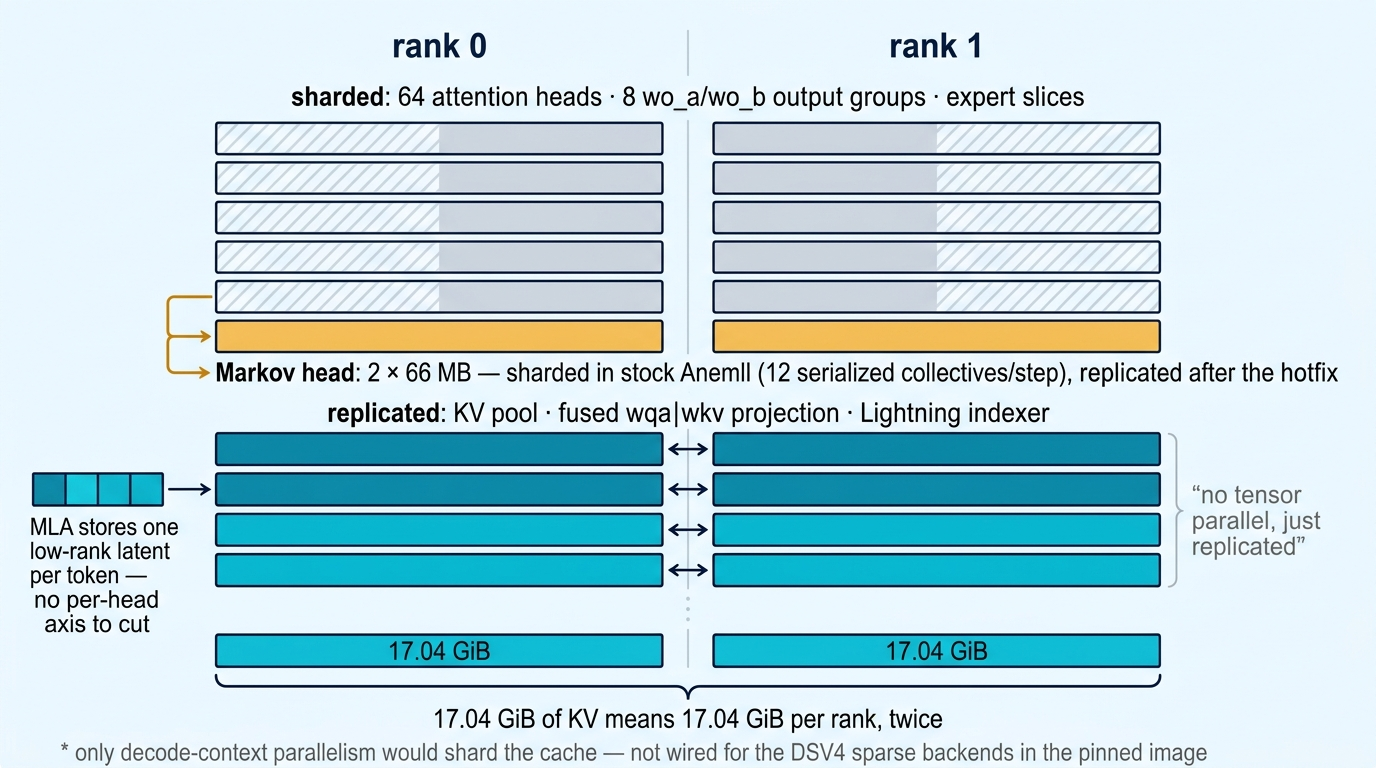
\includegraphics[width=\textwidth]{figures/ch03-tp2-split.png}
\caption{Tensor parallelism shards compute, not cache. Attention heads,
output groups and expert slices are split across the two ranks; the latent
KV pool, the fused projection and the Lightning indexer are held whole on
both, because MLA stores a single low-rank latent per token with no per-head
axis to cut. Every KV capacity figure in this book is therefore a per-rank
figure the cluster pays for twice.}
\label{fig:tp2-split}
\end{figure}

The layers are threaded together by hyper-connection (``mHC'') residual
streams: several parallel residual lanes with a pre/post mixing op around each
attention and FFN block, fused between layers. This detail matters to serving
because the DSpark drafter must capture per-layer features, and collapsing the
mHC streams early breaks the fused chain --- the origin of the deferred-capture
machinery described in \Cref{sec:model-dspark}.

\subsection{Hash-routed MoE on layers 0--2}

Layers 0--2 carry MoE blocks with \emph{no router GEMM}. Expert choice is a
pure table lookup, \code{gate.tid2eid[token_id]}: the token's vocabulary id
selects its experts. This is why the FFN forward signature takes
\code{input_ids} --- a fact that ripples surprisingly far. The multimodal
runner ordinarily drops \code{input_ids} once embeddings exist; Vision-Exp had
to force \code{requires_raw_input_tokens = True} to keep hash routing alive
(\Cref{sec:model-vision}). Every other MoE layer routes with a learned gate
plus a noaux-tc correction bias, top-6 of 256 routed experts, plus one shared
expert that always runs.

\subsection{Quantization: FP8 weights, MXFP4 experts}

The checkpoint metadata says FP8 weights, and the attention/dense linears are
FP8 with $128\times128$ block scales. The 256 routed experts, however, ship in
\code{fp4_e8m0_k32}: MXFP4 values with power-of-two E8M0 scales per 32-element
block. On the GB10 boards the b12x MoE backend consumes this as W4A16
(dequantize to bf16, then MMA) because its NVFP4 tensor-core path accepts only
\code{modelopt_nvfp4}-format weights --- a kernel-level gap
\Cref{ch:perf} quantifies for prefill. Expert scale tensors are loaded with
\code{view(uint8)} rather than numeric casts, because a dtype conversion would
destroy the raw exponent bytes.

\begin{figure}[htbp]
\centering
\begin{tikzpicture}[node distance=5mm and 15mm]
  % --- target stack (left column) ---
  \node[hbbox, minimum width=58mm] (embed)
    {Embedding (vocab 129{,}280)};
  \node[hbnode, minimum width=58mm, below=of embed] (early)
    {\textbf{Layers 0--2}\\[1pt]
     {\scriptsize MLA (layers 0--1 SWA-only)}\\
     {\scriptsize MoE hash-routed: tid2eid[token\_id]}};
  \node[hbnode, text width=56mm, below=of early] (mid)
    {\textbf{Layers 2--42} (alternating)\\[1pt]
     {\scriptsize 21$\times$ C4A: Lightning indexer $\to$ top-512 sparse MLA}\\
     {\scriptsize 20$\times$ C128A: coarse compressed MLA}\\
     {\scriptsize each + MoE: 256 routed top-6 + 1 shared}};
  \node[hbbox, text width=54mm, align=center, below=of mid] (lmhead)
    {hc\_head collapse $\to$ lm\_head\\{\scriptsize (bf16, sharded)}};
  \node[hbnode, minimum width=58mm, below=of lmhead] (verify)
    {sample + verify draft block\\{\scriptsize (rejection sampling)}};
  % --- drafter (right column) ---
  \node[hbfaint, minimum width=44mm, right=of mid] (capture)
    {feature capture at\\dspark\_target\_layer\_ids\\{\scriptsize mHC streams mean-pooled}};
  \node[hbpatch, minimum width=44mm, below=6mm of capture] (draft)
    {\textbf{DSpark draft block}\\[1pt]
     {\scriptsize stacked mtp stages (1 or 3)}\\
     {\scriptsize one non-causal parallel pass}\\
     {\scriptsize over [anchor $|$ noise $\times$ $k$]}};
  \node[hbpatch, minimum width=44mm, below=6mm of draft] (markov)
    {Markov head, rank 256\\{\scriptsize logits += W1[prev]\,W2$^{\top}$, left-to-right}};
  % --- arrows ---
  \draw[hbflow] (embed) -- (early);
  \draw[hbflow] (early) -- (mid);
  \draw[hbflow] (mid) -- (lmhead);
  \draw[hbflow] (lmhead) -- (verify);
  \draw[hbarrow, dashed] (mid.east) -- (capture.west)
    node[hblabel, midway, font=\tiny, align=center, fill=white,
         inner sep=1pt] {stable\\buffers};
  \draw[hbarrow] (capture) -- (draft);
  \draw[hbarrow] (draft) -- (markov);
  \draw[hbok] (markov.south) -- ++(0,-4mm) -|
    node[hblabel, pos=0.25, below] {$k$ draft tokens} (verify.south);
  \draw[hbarrow, dashed] (verify.west) -- ++(-13mm,0) |- (embed.west)
    node[hblabel, pos=0.5, above=1mm, align=center] {accepted\\tokens};
  \begin{scope}[on background layer]
    \node[hbgroup, fit=(capture)(draft)(markov),
      label={[hbtitle]above:DSpark drafter (no vLLM KV)}] {};
  \end{scope}
\end{tikzpicture}
\caption{DeepSeek-V4-Flash as served: the 43-layer target stack (left) with the
DSpark drafter (right) hanging off captured target-layer features. The drafter
predicts a whole block in one non-causal pass and keeps its own sliding-window
state outside the vLLM KV cache.}
\label{fig:model-block}
\end{figure}

\section{The sparse attention stack}
\label{sec:model-sparse}

Full attention over a million tokens is not an option on this hardware, and
V4-Flash does not attempt it. Instead every layer carries one of three
attention flavors, scheduled across the stack: layers 0--1 are sliding-window
only (SWA, window 128); layers 2--42 alternate between 21 \emph{C4A} layers
and 20 \emph{C128A} layers. The ``C$n$'' names are compression ratios: a C4
layer maintains a compressed KV row for every 4 tokens, a C128 layer one per
128 tokens. All layers additionally keep the 128-token sliding window, so
recent context is always attended exactly. The whole stack is one bargain
repeated across 43 layers: recent tokens attended exactly, older tokens kept
only in compressed form at one of two ratios, and on the C4 layers only the
compressed rows a scoring module judges worth reading
(\Cref{fig:attention-flavors}).

\subsection{The Lightning indexer}

On the 21 C4A layers, a query does not attend to all compressed rows. A
separate scoring module --- the Lightning indexer --- selects the
\code{index_topk} = 512 compressed rows each query is allowed to read. It has
64 index heads of 128 dims and its own quantized K cache (132\,B per
compressed token per C4 layer). The module is also deliberately \emph{not}
tensor-parallel: the source comments read ``no tensor parallel, just
replicated,'' so \code{wq_b} and \code{weights_proj} are
\code{ReplicatedLinear} and every rank scores all 64 heads against the
entire compressed key range.

The consequence of that replication is quadratic scoring work that no rank
can share. At short context this is noise; at 900K tokens of prompt the
indexer is the dominant prefill cost --- about 875 prefill \tokspersec{} on a
899{,}994-token prompt versus 2{,}563 at 2K. That is why \Cref{ch:patches} ships an
opt-in sequence-parallel indexer prefill.

There is also a window in which the whole apparatus provably does nothing.
When $\text{max\_seq\_len} \le 512 \times 4 = 2048$ tokens, \emph{every}
compressed candidate fits in the top-512: score-and-select cannot change the
answer, so the entire pipeline is a no-op. That is not a curiosity --- it is
the trigger window for the upstream \ghissue{49486} shortcut backport, which
exists precisely because short-context requests were paying full price for a
selection that could not select.

C128A layers do not run the indexer; their candidate indices are computed at
metadata-build time. The compressed rows themselves are written by a
Python-side CuTeDSL kernel
(\code{SparseAttnCompressNormRopeStoreC4Kernel}, with a Triton fallback),
while the sliding-window rows are written by a compiled C++ op inside vLLM's
\code{_C} extension. That split matters when you contemplate changing the
row format: only one of the two writers is modifiable without rebuilding
vLLM.

\begin{figure}[htbp]
\centering
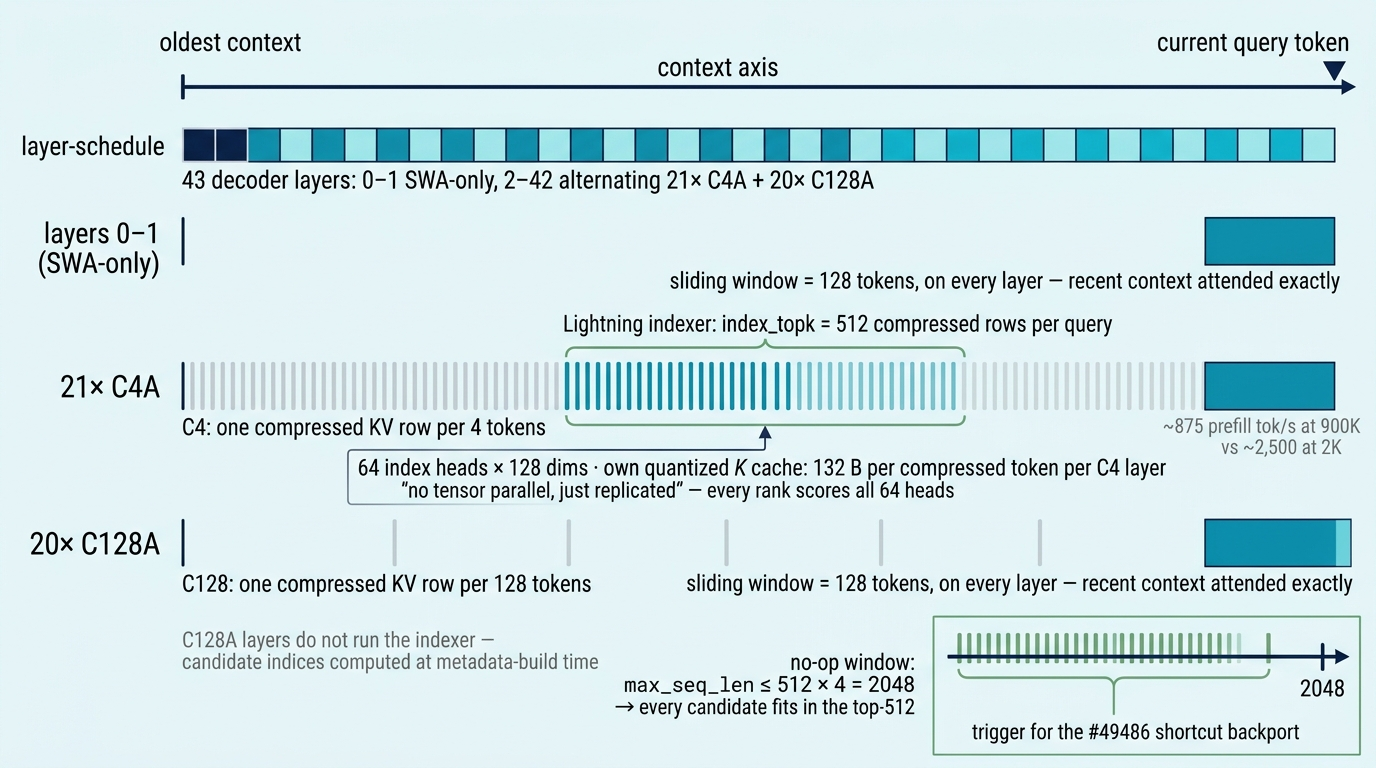
\includegraphics[width=\textwidth]{figures/ch03-attention-flavors.png}
\caption{One bargain, repeated 43 times. Every layer attends the most recent
128 tokens exactly; older context survives only as compressed rows --- one
per 4 tokens on the 21 C4A layers, one per 128 on the 20 C128A layers ---
and on C4A layers a query may read only the 512 rows the Lightning indexer
selects. Below 2{,}048 tokens every candidate already fits in the top-512,
so the selection provably cannot change the answer.}
\label{fig:attention-flavors}
\end{figure}

\subsection{The 584-byte KV row}
\label{sec:model-kvrow}

Every stored token row --- compressed or sliding-window --- occupies exactly
584 bytes, fixed by FlashInfer's \code{KVCacheTraits<DSV4>}
(\code{KV_GMEM_STRIDE = 584}). \Cref{fig:kv-row} maps the bytes.

\begin{figure}[htbp]
\centering
\begin{tikzpicture}[x=0.0235cm, y=1cm]
  % main bar
  \draw[draw=hbSteel, thick, fill=hbGreen!12] (0,0) rectangle (448,0.95);
  \draw[draw=hbSteel, thick, fill=hbBlue!8]   (448,0) rectangle (576,0.95);
  \draw[draw=hbSteel, thick, fill=hbAmber!25] (576,0) rectangle (584,0.95);
  % quant tile ticks inside NoPE region (every 64 values)
  \foreach \xx in {64,128,192,256,320,384} {
    \draw[hbSteel!50, dash pattern=on 1pt off 1pt] (\xx,0) -- (\xx,0.95);
  }
  \node at (224,0.475) {\small 448\,B NoPE: 448 $\times$ fp8 e4m3};
  \node[align=center, font=\scriptsize] at (512,0.475) {128\,B RoPE:\\64 $\times$ bf16};
  % byte offsets
  \node[hblabel, below] at (0,-0.05) {0};
  \node[hblabel, below] at (448,-0.05) {448};
  \node[hblabel, below] at (566,-0.05) {576};
  \node[hblabel, below] at (596,-0.05) {584};
  % tile brace
  \draw[decorate, decoration={brace, amplitude=4pt}, hbSteel]
    (0,1.05) -- (448,1.05)
    node[hblabel, midway, above=4pt]
    {7 quant tiles of 64 values, one UE8M0 scale each (scales live in the footer)};
  % footer zoom
  \draw[hbSteel!70] (576,0) -- (300,-1.5);
  \draw[hbSteel!70] (584,0) -- (584,-1.5);
  \draw[draw=hbSteel, thick, fill=hbAmber!25] (300,-2.3) rectangle (584,-1.5);
  \foreach \i in {1,...,6} {
    \draw[hbSteel] ({300+\i*35.5},-2.3) -- ({300+\i*35.5},-1.5);
  }
  \draw[hbSteel, thick] ({300+7*35.5},-2.3) -- ({300+7*35.5},-1.5);
  \foreach \i/\lbl in {0/S0,1/S1,2/S2,3/S3,4/S4,5/S5,6/S6} {
    \node[font=\scriptsize] at ({300+\i*35.5+17.7},-1.9) {\lbl};
  }
  \node[font=\scriptsize] at ({300+7*35.5+17.7},-1.9) {pad};
  \node[hblabel, below] at (442,-2.4)
    {8\,B footer: 7 UE8M0 scales (uint8, exponent+127) + 1 pad byte};
\end{tikzpicture}
\caption{The 584-byte per-token KV row used by both \code{fp8_ds_mla} and
\code{nvfp4_ds_mla}: 448 fp8 e4m3 NoPE values in seven 64-value quant tiles,
64 bf16 RoPE values kept at full precision, and an 8-byte footer holding the
seven power-of-two UE8M0 tile scales plus one pad byte.}
\label{fig:kv-row}
\end{figure}

The design encodes two numerics decisions. First, only the NoPE (non-rotary)
dimensions are quantized to fp8; the 64 RoPE dimensions stay bf16, because
positional phase at million-token context is the last thing you want to
degrade. Second, the scales are UE8M0 --- pure powers of two, computed as
$2^{\lceil \log_2(\mathrm{absmax}/448) \rceil}$ and stored as
$\mathrm{exponent}+127$ in a uint8 --- so dequantization is an exponent add,
not a multiply.

\begin{hblesson}
This row is what the \ghissue{22} incident from the chapter opening was
about: \code{nvfp4_ds_mla} and \code{fp8_ds_mla} store these same 584 bytes,
and there is no 4-bit KV cache in this stack today. The lesson generalizes:
when two configuration strings are documented as byte-identical, audit every
string comparison that treats them differently. A genuine 4-bit row
($\approx$292--390\,B) is a designed-but-unbuilt future
(\repofile{docs/CLAUDE/item8-fp4-kv-design.md}); it would buy roughly
+50\,\% KV tokens.
\end{hblesson}

\subsection{Per-token byte accounting and KV groups}

This subsection is the byte ledger --- reference material, not narrative.
Skim it on first read and return when you need to size a deployment.

Because C4 layers store one row per 4 tokens and C128 one per 128, the
\emph{amortized} physical cost per context token is far below 584\,B per layer
(\Cref{tab:kv-bytes}). The allocator sees something different. vLLM's hybrid
allocator requires every KV group to use the same page size in bytes, and all
four groups land on $64 \times 584 = 37{,}376$\,B pages: one
\code{MLAAttentionSpec} group (block 256 tokens) plus three
\code{SlidingWindowMLASpec} groups (blocks 64/4/8, the latter two serving the
draft layers). The published headline ``2.33\,M tokens in 17.04\,GiB''
($\approx$7.8\,KB/token) is allocator accounting across those groups, not
physical row cost.

\begin{table}[htbp]
  \centering\small
  \caption{Physical KV bytes per context token at long context (per rank;
  TP=2 replicates everything on both ranks).}
  \label{tab:kv-bytes}
  \begin{tabular}{@{}lrl@{}}
    \toprule
    Component & Bytes/token & Derivation \\
    \midrule
    C4 compressed rows & $\approx$3.07\,KB & 21 layers $\times$ 584/4 \\
    C128 compressed rows & $\approx$0.09\,KB & 20 layers $\times$ 584/128 \\
    Indexer K cache & $\approx$0.69\,KB & 21 layers $\times$ 132/4 \\
    SWA windows & --- & per-sequence constant, $\approx$3.4\,MB/seq \\
    \bottomrule
  \end{tabular}
\end{table}

\section{DSpark speculative decoding at the model level}
\label{sec:model-dspark}

Everything to this point has described what the target stack stores and
reads; the other half of every decode step is the passenger grafted onto
it. DSpark is the checkpoint's built-in speculative decoder. Mechanically it is a
descendant of MTP (multi-token prediction), but with a twist that reshapes the
serving math. The \code{mtp.N.*} draft stages are \emph{stacked} into one
non-causal draft backbone that predicts a whole \code{dspark_block_size} = 5
token block in a single parallel pass, rather than re-running one MTP layer
per drafted token. The scheduler-facing details live in \Cref{ch:specdecode};
here is the model anatomy. That anatomy has four pieces: where the drafter's
input comes from, how many stages it actually has, what a single block pass
computes, and where its state lives. The last is the one later bugs turn on,
because that state sits outside the KV cache the engine knows how to manage.

Two of the design decisions read best as reasoning rather than inventory.
The drafter's \emph{input} is not the target's final hidden state. During
the target forward, the mHC stream state after each layer listed in
\code{dspark_target_layer_ids} is collapsed (mean over streams) and copied
into a stable-address buffer allocated outside the CUDA-graph pool, so that
captured graphs refresh it at replay; the drafter reads that concatenated
mid-stack feature buffer. And the drafter's \emph{depth} is not taken on
faith. 0731 declares \code{num_nextn_predict_layers} = 1 where Vision-Exp
declares 3, but the overlay's \code{DSparkModelSpec.from_hf_config} does
not take that field on trust: it infers the true stage count from the
contiguous \code{mtp.N.*} weight namespace, its source comment noting that
DSpark releases still report \code{num_nextn_predict_layers=1}, ``so the
weight map is the reliable source for the DSpark draft depth.'' The
transferable rule: count the
weights, not the config's claims --- a checkpoint's tensors cannot lie
about their own existence.

\begin{description}
  \item[The block pass.] \code{draft()} builds a $[B, \mathrm{block}]$ input:
  the anchor token (last accepted token) first, then noise tokens, at
  positions $\mathrm{anchor} + [0, k)$. One forward of the stacked draft
  layers produces features for every position at once.
  \item[The Markov head.] Decoding the block is left-to-right, but cheap: at
  each position the base draft logits get a low-rank bias
  $W_1[\mathrm{prev\_token}] \, W_2^{\top}$ with rank
  \code{dspark_markov_rank} = 256 --- a learned bigram correction. Both
  matrices are $129{,}280 \times 256$ bf16, 66\,MB each. Stock Anemll shards
  them tensor-parallel, which costs 12 serialized collectives per decode step
  in the six-step draft loop. The replicate-Markov-head hotfix
  (\Cref{ch:patches}) makes them plain replicated modules, because 66\,MB is
  trivially affordable next to a 128\,GB unified board.
  \item[Draft state.] The drafter's KV is \emph{not} vLLM KV cache. Each draft
  layer owns a per-request sliding window of projected target features
  (\code{main_kv_cache}); the proposer registers no KV layers and sets
  \code{block_size = 1}. This design is what made the batch-condensation bug
  of the Keys concurrency patch possible --- state keyed by batch row rather
  than request id --- covered in \Cref{ch:bugs}.
\end{description}

The launcher serves this with $k=5$ or $k=6$ speculative tokens
(\code{MTP_NUM_TOKENS}, default 6). Vision-Exp exposes a config trap.
vLLM's \code{SpeculativeConfig} requires $k$ divisible by the draft stage
count ``for MTP module reuse'' --- a rule that is meaningless for DSpark's
stacked block, but with 3 stages it forces $k = 6$, one more noise query
than the 5-token block was trained with. The opt-in, SHA-pinned
\repofile{patches/hotfix-vllm-dspark-block-k.py} exempts
\code{method="dspark"} from the rule.

\begin{lstlisting}[language=bash]
# compose argv (TP=2 lane), the model-level spec-decode knobs:
--speculative-config '{"method":"dspark",
                       "num_speculative_tokens":6,
                       "draft_sample_method":"probabilistic"}'
\end{lstlisting}

Acceptance behavior is strongly prompt-dependent, and the repository measured it
honestly. On numbered-word probes the audited healthy curve is per-position
acceptance 0.92 / 0.74 / 0.60 / 0.41 / 0.28 / 0.21 --- about 48\,\% of drafted
tokens accepted, $\approx$3.9 tokens per step at $k=6$. On natural prose the
same stack accepts only $\approx$25\,\% with position-0 agreement
0.66--0.69, and a vision-lane \code{/metrics} snapshot showed 23.7\,\%
acceptance with positions 2--5 nearly dead. Drafts are verified by the target
with rejection sampling, so acceptance moves throughput, never correctness.
\Cref{fig:dspark-block} draws one block and the decay along it.

\begin{figure}[htbp]
\centering
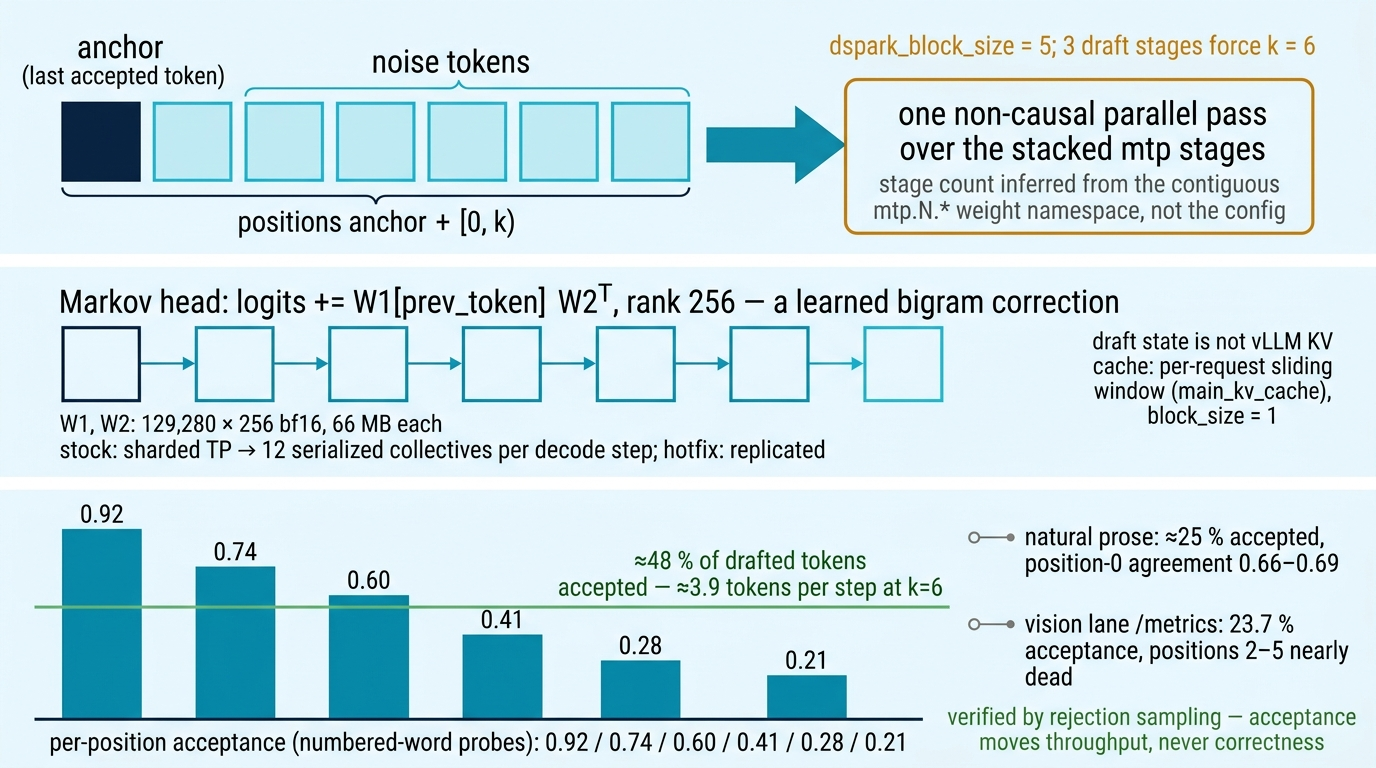
\includegraphics[width=\textwidth]{figures/ch03-dspark-block.png}
\caption{One DSpark block. The drafter builds an anchor token plus $k$ noise
tokens, produces features for all of them in a single non-causal pass, and
decodes them left-to-right through a rank-256 bigram bias; the target then
verifies the whole block in one pass. Acceptance decays steeply with position
and depends heavily on the workload --- the audited healthy curve yields
roughly 3.9 tokens per step, while natural prose and the vision lane accept
about a quarter of what is drafted.}
\label{fig:dspark-block}
\end{figure}

\section{Vision-Exp: a vision tower by startup hotfix}
\label{sec:model-vision}

The weakest of those acceptance numbers came from the vision lane --- a
lane this stack was never originally built to have.
The published 0731 checkpoint is text-only: no vision processor, projector, or
tower. DeepSeek-V4-Flash-\emph{Vision-Exp} ships a 32-layer ViT plus an
Aligner (a $3\times$ spatial downsample-and-project into the 4096-dim LLM
hidden size) and an in-vocabulary image placeholder token,
\code{<|deepseek_image|>} (token id 129{,}264).

The pinned Anemll image knows nothing about any of this, so the repository adds
vision \emph{at container start}.
\repofile{patches/hotfix-dsv4-vision-exp.py} appends a fail-closed import hook
to the stock model file, which pulls in the \repofile{patches/vision_exp/}
package and monkey-patches the three stock classes --- tower construction,
weight-name mapping, the multimodal processor, and MoE routing --- without
editing their source. Two limits are worth separating. The processor advertises support for 16
images per request, but the shipped serve flag admits only 8
(\code{--limit-mm-per-prompt} \code{{"image":8}}, \Cref{ch:profile}), so 8
is the number a client actually meets. The rest of the envelope: at most
384 LLM tokens per image (\code{vision_max_n_token}), images in \code{user}
messages only --- \code{system} and \code{assistant} return HTTP 400 --- and
no video, because the official weights have no video encoder and a GIF
decodes as a single still frame.

Two model-level mechanisms in this overlay are worth teaching, and both
follow from that bolt-on construction: the runtime underneath does not know
images exist, so each is a place where image rows must behave differently
from text rows without the surrounding machinery noticing --- the second of
them drawn in \Cref{fig:image-cache}.

\paragraph{\code{bias_vl} routing for image tokens (issue \ghissue{175}).}
Vision-Exp ships a second MoE correction bias,
\code{e_score_correction_bias_vl}, for image rows --- and image rows must skip
the hash table (an image placeholder is a real vocabulary id; looking up
\code{tid2eid[129264]} would route it like a text token). The naive
implementation scans token ids at each of the 43 gates, a GPU$\to$CPU sync per
gate. The shipped design classifies the batch once per forward (text / image /
mixed, derived from a sum the multimodal merge already reads), publishes the
verdict through the forward context, and splits mixed batches so each
partition routes with its own bias. A hard rule protects CUDA graphs: while
stream capture is active the wrapper always takes the original path, because a
captured graph must never resolve a routing kind.

\begin{hbwarstory}
\textbf{Issue \ghissue{172}: the position-dependent image block.} Vision-Exp
pads every image block so it starts on a 4-token boundary:
$4 - 1 - (\mathrm{start\_pos} \bmod 4)$ pad tokens are prepended, so the
\emph{total} block length depends on where in the prompt the image lands. A
$40\times19$ ViT grid becomes 122 core tokens plus 0--3 pad --- 122 to 125
tokens for the same pixels. vLLM's encoder cache, however, keyed entries by
content hash alone. An image first encoded at one alignment could be reused at
another, yielding ``125 placeholders vs 124 embeds'' and a scatter mismatch.
The fix salts the multimodal hash with the block's token count
(\code{salt_mm_image_hash}), bypasses the content-only processor cache for
image requests, and leaves a runtime tripwire: whenever placeholder and
embedding counts disagree, the embedding merge raises with the
\ghissue{172} explanation attached. Positional context changing the \emph{size} of an
embedded object is exactly the kind of invariant a generic cache will violate
silently.
\end{hbwarstory}

\begin{figure}[htbp]
\centering
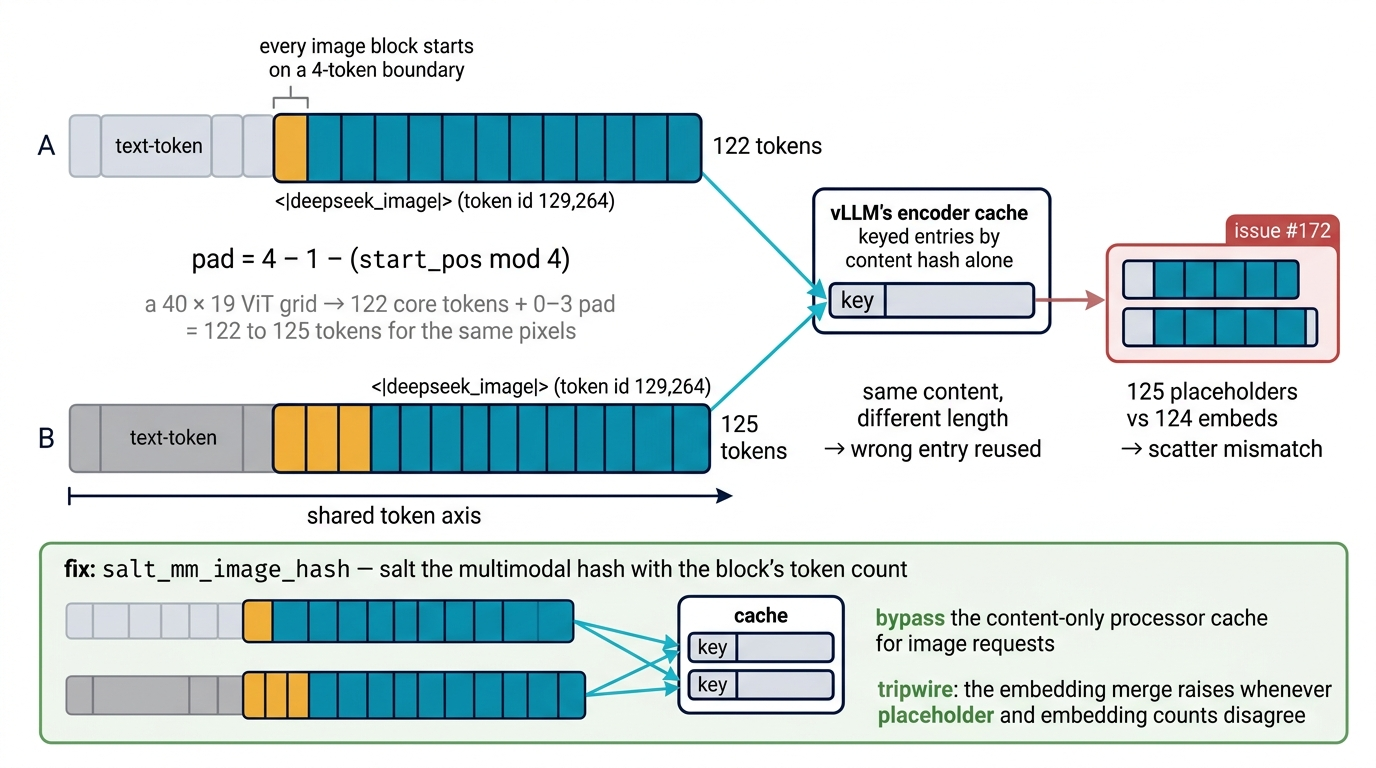
\includegraphics[width=\textwidth]{figures/ch03-image-block-cache.png}
\caption{Positional context changing the size of an embedded object.
Vision-Exp pads each image block to a 4-token boundary, so identical pixels
occupy 122 to 125 tokens depending on where the image lands in the prompt ---
while vLLM's encoder cache keyed entries by content hash alone and happily
reused an entry across alignments. Salting the hash with the block's token
count (\code{salt_mm_image_hash}) separates the two, and a runtime tripwire
catches any residual placeholder/embedding disagreement (\ghissue{172}).}
\label{fig:image-cache}
\end{figure}

\section{The encoding layer: a Python encoder instead of a chat template}
\label{sec:model-encoding}

Images, tool calls, and thinking controls all cross into and out of the
model through one last checkpoint-supplied mechanism.
The model card ships no Jinja chat template. Instead the checkpoint carries an
\code{encoding} package --- \repofile{encoding/encoding_dsv4.py} --- that
defines message rendering \emph{and} output parsing. The launcher sets
\envvar{DSPARK_ENCODING_FILE} to that file inside the container and installs
it into vLLM before import on both ranks (\code{--tokenizer-mode deepseek_v4});
request controls such as \code{chat_template_kwargs.thinking} flow through
vLLM's custom tokenizer wrapper into the Python encoder. The install also
repairs two encoder bugs: pre-0731 wrappers that mapped \code{low} reasoning
effort to \code{high}, and issue \ghissue{21}, where
\code{encode_arguments_to_dsml} only accepted JSON \emph{strings} for tool
arguments. Under \ghissue{21}, a replayed history with dict-typed arguments
was silently wrapped as \code{{"arguments": ...}}, poisoning every later
tool turn.
\Cref{fig:dsml-flow} traces the round trip.

\begin{figure}[htbp]
\centering
\adjustbox{max width=\textwidth}{%
\begin{tikzpicture}[node distance=4mm and 7mm]
  \node[hbhost, minimum width=30mm] (msgs)
    {messages JSON\\{\scriptsize roles, tools, thinking kwarg}};
  \node[hbbox, minimum width=34mm, right=of msgs] (enc)
    {encoding\_dsv4.py\\{\scriptsize renders DSML + <think>}};
  \node[hbgpu, minimum width=26mm, right=of enc] (engine)
    {vLLM engine\\{\scriptsize token ids in/out}};
  \node[hbbox, minimum width=34mm, right=of engine] (parse)
    {deepseek\_v4 parsers\\{\scriptsize reasoning + tool-call}};
  \node[hbhost, minimum width=28mm, below=8mm of parse] (out)
    {reasoning\_content\\+ tool\_calls[]};
  \draw[hbflow] (msgs) -- (enc);
  \draw[hbflow] (enc) -- (engine);
  \draw[hbflow] (engine) -- (parse);
  \draw[hbok] (parse) -- (out);
  \node[hblabel, align=center, anchor=north east]
    (dsmlfail) at ([xshift=-2mm,yshift=-8mm]parse.south west)
    {malformed DSML syntax\\$\to$ parse fails $\to$ no tool\_calls};
  \draw[hbfail] ([yshift=-1mm]parse.south west) to[bend right=15] (dsmlfail.north);
\end{tikzpicture}%
}
\caption{The encoding round trip: a checkpoint-supplied Python encoder renders
messages into DSML-marked tokens, and the paired \code{deepseek_v4} parsers
must recover structure from the output. Any syntax corruption breaks the
structured \code{tool_calls} field even when the payload was right.}
\label{fig:dsml-flow}
\end{figure}

\subsection{Thinking modes}

Reasoning effort accepts \code{off}, \code{low}, \code{high}, or \code{max};
the recipe defaults \envvar{DEFAULT_THINKING} to \code{low}, which opens a
\code{<think>} block but adds no effort instruction (matching the model's
intended base mode). \code{high}/\code{max} add instruction prefixes.

\begin{hbwarning}
\code{max_tokens} counts \emph{think plus answer}. Reasoning is generated
inside the same completion as the visible reply, so a request with
\code{DEFAULT_THINKING=max} and a small \code{max_tokens} spends the whole
window inside \code{<think>} and returns an empty-looking answer. The repository's
own benchmark notes flag this: \repofile{scripts/benchmark-0731.py} uses
natural completions without forcing \code{thinking=false}, and its numbers are
not comparable to the capped, thinking-off matrix for exactly this reason.
Budget reasoning explicitly (the per-request \code{thinking_token_budget}
parameter exists for this) rather than trusting \code{max_tokens} to bound the
visible answer.
\end{hbwarning}

\subsection{DSML tool calls and the temperature asymmetry}

Tool calls are emitted as DSML markup inside the token stream (shown here with
ASCII pipes; the real markers use a wide-bar glyph):

\begin{lstlisting}
<|DSML|tool_calls>
  <|DSML|invoke name="get_weather">
    <|DSML|parameter name="city">Paris</|DSML|parameter>
  </|DSML|invoke>
</|DSML|tool_calls>
\end{lstlisting}

The \code{deepseek_v4} tool-call parser turns this into the structured
\code{tool_calls} field of the Chat Completions response --- and it is here
that a benchmark can tell you the model got worse when it hadn't. On tool
benchmarks at temperature 1.0, the same weights score lower under this vLLM
profile than under ds4, the sibling single-Spark engine. Part of that loss is
a mechanical serving artifact rather than a model-quality signal, and
\repofile{docs/DSML_SYNTAX_TEMP_ASYMMETRY.md} documents the mechanism ---
while proposing a temperature-0 rerun to establish how much of the gap it
actually accounts for.

The asymmetry: ds4 forces \code{temperature=0} while the model emits DSML
\emph{syntax} tokens --- tags, invoke headers, JSON punctuation --- and
applies the request's sampling parameters only to argument \emph{payloads}.
vLLM has no per-region temperature mechanism: at \code{temperature=1.0}
every structural token is a full-temperature sample. A single derailed
structural token anywhere in the call makes the DSML unparseable. The
response then carries no \code{tool_calls}, and a benchmark that reads only
the structured field scores it as ``no tool call.''

The document earns its verdict by ruling out the tempting alternative
explanations (KV precision, spec decode, weight format), then lists
mitigations from cheapest to hardest. The cheapest: run tool benchmarks at
temperature 0 as a diagnostic. At the far end sit a DSML structural-tag
grammar, or a logits processor that forces argmax inside syntax regions ---
effectively porting ds4's hand-written C logic.

The generalization outlives DSML. When structure and payload are sampled at
one temperature, a benchmark that reads only the structured field is partly
scoring the decoder's syntax rather than the model's judgment.

\section{Checkpoint variants}
\label{sec:model-variants}

Like the byte ledger, this short section is reference rather than
narrative; return to it whenever two measurements disagree and you suspect
the checkpoints differ. Three checkpoint lineages appear throughout this
book; conflating them invalidates comparisons, so the repository pins them
explicitly (\Cref{tab:checkpoints}).

\begin{table}[htbp]
  \centering\footnotesize
  \caption{Checkpoint lineages served by the repository.}
  \label{tab:checkpoints}
  \begin{tabular}{@{}>{\raggedright\arraybackslash}p{3.4cm}>{\raggedright\arraybackslash}p{4.6cm}>{\raggedright\arraybackslash}p{5.6cm}@{}}
    \toprule
    Lineage & Pin & Notes \\
    \midrule
    0731 (text-only) &
    \code{deepseek-ai/DeepSeek-V4-Flash-0731} @ \code{9e165c30}\ldots &
    default \envvar{DSPARK_REVISION}; supersedes the preview
    \code{DeepSeek-V4-Flash-DSpark} checkpoint; 1 draft stage; the published
    two-Spark benchmark lane \\
    Vision-Exp (official) &
    \code{deepseek-ai/DeepSeek-V4-Flash-Vision-Exp} @ \code{86f746b3}\ldots &
    ViT + Aligner; 3 draft stages; served via the vision patch train \\
    Vision-Exp (Keys abliterated) &
    \code{drowzeys/keys-DeepSeekV4Flash-Vision-EXP-ablit}, unpinned by default
    (\envvar{DSPARK_REVISION_ABLITERATED}) &
    HF-gated; selected with \envvar{ABLITERATED}=1; applied as a 26-shard
    delta overlay onto the official snapshot \\
    \bottomrule
  \end{tabular}
\end{table}

The prepare script resolves official versus abliterated from a CLI flag, an
environment variable, or an interactive prompt, then records the choice back
into \repofile{.env.dspark}. It also guards the operational footgun: if a
pinned revision is not already in the HF cache on \emph{both} nodes, a
restart quietly becomes a $\approx$155\,GB download. Everything else in this chapter ---
architecture, KV layout, DSpark structure, encoder --- is common across the
three; what changes is the draft stage count, the vision tower, and the
weights themselves.

\FloatBarrier
The checkpoint is no longer a thing that gets loaded; it is a set of budgets
and invariants the rest of the stack negotiates with. ``17\,GiB of KV'' is a
per-rank figure the cluster pays for twice, because MLA leaves tensor
parallelism no per-head axis to cut --- the cache replicates while the
compute shards. And the names attached to those budgets are not evidence:
two KV dtypes that share every one of their 584 bytes, a config field that
misreports the drafter's stage count, a top-512 selection that provably
cannot select below 2{,}048 tokens, and a benchmark score that was partly
measuring DSML syntax rather than the model's judgment.

\section*{Takeaways}

\begin{itemize}
  \item MLA shards compute, not cache: every TP rank holds the full KV pool,
  so capacity quotes are per rank, replicated.
  \item The KV row is 584 bytes, and \code{nvfp4_ds_mla} is byte-identical
  to \code{fp8_ds_mla} --- when two config strings share bytes, audit every
  comparison that treats them differently (\ghissue{22}).
  \item DSpark predicts a whole block in one non-causal pass over
  anchor-plus-noise, decoded through a rank-256 Markov bias, with its draft
  state outside the vLLM KV cache.
  \item Layers 0--2 route MoE by token-id hash, which is why the FFN needs
  raw \code{input_ids} and image tokens need \code{bias_vl} routing that
  skips the table.
  \item Checkpoint lineage changes the draft-stage count, and the stage
  count alone changes the legal values of $k$ --- so count the weights, not
  the config's claims.
\end{itemize}

\chaptertransition{Every mechanism in this chapter reaches the running
engine as a single number or string in the launch command: the KV dtype
whose name selects a kernel, the block size the row layout implies, the
speculative $k$ the stage count constrains, the sequence count the shared
pool must absorb. None of those values is independent of the others: the
draft stage count fixes the legal $k$, and $k$ fixes the shape of every
decode step the engine has to capture. The next chapter reads
the entire \code{vllm serve} argv in that light --- the ceilings, the
KV-pool arithmetic behind the 1M claim, the thinking budgets that decide
whether an answer arrives at all --- and it opens on the smallest possible
mistake: a flag set to 42, the exactly correct product of six sequences and
$k+1$ tokens, which cost 12\,\% of six-stream throughput precisely because
nobody rounded it up.}
